% Szoftprojlab
% ===========================================================================
%
\chapter{Analízis modell kidolgozása 1}

\thispagestyle{fancy}

\section{Objektum katalógus}

\subsection{Játékos}
Három vagy több van belőle. Körökre bontva teszik a dolgukat. Saját körükben tudnak mozogni, különböző tárgyakat használni vagy a speciális képességüket használni. A játék megnyeréséhez szükséges rakétapisztoly alkatrészek összegyűjétse a feladatuk. Ha vízbe esnek, vagy kihűlnek akkor a játéknak vége.

\subsection{Jégtábla}
Ilyenek alkotják a játékos számára a játékteret, ezeken lehet mozogni. Jégtáblák tartalmazhatnak tárgyakat amelyeket ki lehet ásni. Az instabil jégtábla képes vízbe ejteni a rajta állókat, ha túl sokan vannak. A jégtáblán lehet hó. Néha lehet rajta hóvihar, mely csökkenti a rajta állók testhőjét

\subsection{Kötél}
Ennek segítésével ki lehet húzni egy vízbe esett játékost.

\subsection{Búvárruha}
A játékos képes a vízben is mozogni vele, illetve nem veszít testhőt ha vízben tartózkodik.

\subsection{Lapát}
Segítségével 2 egységnyi hó takarítható el, egy egység munkával.

\subsection{Élelem}
Ha a játékos elfogyasztja, a testhője 1-el megnő.

\subsection{Rakétapisztoly Alkatrész}
A játékban 3 darab ilyen megtalálása vezet a játék sikeres befejezéséhez. Az összeszereléshez mindháromnak egy helyen kell lennie.

\subsection{Iglu}
Eszkimó (Játékos) képes építeni, itt átvészelhetőek a hóviharok.

\section{Osztályok leírása}
\subsection{BareHands}
\begin{itemize}
	\item A játékos így ás, ha nincs ásója. A kiválasztott cellán csökkennie kell a hó mennyiségnek ásáskor.
	\item Interfészek:
	\begin{itemize}
		\item DigStrategy
	\end{itemize}
	\item Metódusok:
	\begin{itemize}
		\item bool Dig(Tile t): Csökkenti a tile-on található hó mennyiségét. Minden alkalommal fárasztó az ásás, ezért a visszatérési érték mindig true.
	\end{itemize}
\end{itemize}

\subsection{BareIce}
\begin{itemize}
	\item Ilyen a jégtábla, ha nincs rajta iglu. A jégtáblán nincs védelem a vihar elől.
	\item Interfészek:
	\begin{itemize}
		\item ChillStormStrategy
	\end{itemize}
	\item Metódusok:
	\begin{itemize}
		\item void Chill(Tile t): A paraméterként kapott t Tilen álló játékosok testhője csökken.
	\end{itemize}
\end{itemize}

\subsection{CantRescue}
\begin{itemize}
	\item A játékos nem tudja kihúzni a csapattársát. A játékos ilyen állapotban van, ha nincs nála kötél.
	\item Interfészek:
	\begin{itemize}
		\item RescueStrategy
	\end{itemize}
	\item Metódusok:
	\begin{itemize}
		\item void Rescue(Tile water, Tile land): Mivel a játékos ebben az állapotban nem tudja megmenteni a csapattársát, ez a fv nem csinál vele semmit. 
	\end{itemize}
\end{itemize}

\subsection{ChillStormStrategy}
\begin{itemize}
	\item A jégtábla így hűti viharban a játékosokat. Vihar esetén a játékos testhője csökken, a megvalósított stratégia alapján.
	\item Metódusok:
	\begin{itemize}
		\item abstract void Chill(Tile t): A startégiát megvalósítő elem dolga implementálni mi történik.
	\end{itemize}
\end{itemize}

\subsection{ChillWaterStrategy}
\begin{itemize}
	\item A jégtábla így hűti a vízbe esett játékosokat. Vízben tartózkodás esetén a játékos testhője csökken, a megvalósított stratégia alapján.
	\item Metódusok:
	\begin{itemize}
		\item abstract void Chill(Tile t): A startégiát megvalósító elem dolga implementálni mi történik.
	\end{itemize}
\end{itemize}

\subsection{DigStrategy}
\begin{itemize}
	\item A játékos így ás.	Ásáskor a cellán a hómennyiség csökken.
	\item Metódusok:
	\begin{itemize}
		\item abstract bool Dig(Tile t): A stratégiát megvalósító elem dolga implementálni mi történik ásáskor. Visszaadja, hogy az ásás fárasztó-e.
	\end{itemize}
\end{itemize}

\subsection{DryLand}
\begin{itemize}
	\item A szárazföld nem hűti a játékosokat. A játékos nincsen vízben.
	\item Interfészek:
	\begin{itemize}
		\item ChillWaterStrategy
	\end{itemize}
	\item Metódusok:
	\begin{itemize}
		\item void Chill(Tile t): A stratégia megvalósítása miatt kér be egy t Tile paramétert, a rajta levő játékossal viszont nem csinál semmit, mert az nincs vízben, nem csökkenti testhőjét.
	\end{itemize}
\end{itemize}

\subsection{Empty}
\begin{itemize}
	\item Nincs jégbe fagyott tárgy. Ez az üres eszköz típus, nem képes semmi extra tulajdonságot biztosítani a tulajdonosnak.
	\item Interfészek:
	\begin{itemize}
		\item Item
	\end{itemize}
	\item Metódusok
	\begin{itemize}
		\item void GiveTo(Player p): A paraméterként kapott játékost nem ruházza fel extra tulajdonsággal, mivel épp nincs itt jégbe fagyott tárgy.
	\end{itemize}
\end{itemize}

\subsection{Eskimo}
\begin{itemize}
	\item Játékos fajta. 5 egységnyi testhővel kezd. Képes iglut építeni. A játékos irányítja.
	\item Ősosztályok:
	\begin{itemize}
		\item Player
	\end{itemize}
	\item Metódusok:
	\begin{itemize}
	\item void BuildIgloo(): Épít egy iglut a mezőre, amin áll. Az iglu megvéd majd a hóvihartól. Beállítja a mező hóvihar stratégiáját Iglusra.
	\end{itemize}
\end{itemize}

\subsection{Food}
\begin{itemize}
	\item Élelem, amit a játékos meg tud enni, hogy növelje a testhőjét. Élelem a pályán lesz található.
	\item Interfészek:
	\begin{itemize}
		\item Item
	\end{itemize}
	\item Metódusok:
	\begin{itemize}
		\item void GiveTo(Player p): A paraméterként kapott játékos kap egy élelmet, az bekerül az élelemtárolójába.
	\end{itemize}
\end{itemize}

\subsection{FoodStore}
\begin{itemize}
	\item A játékos ebben a zsebben tárolja az élelmet.
	\item Attribútumok:
	\begin{itemize}
		\item count: int: Hány élelem van a játékosnál.
	\end{itemize}
	\item Metódusok:
	\begin{itemize}
		\item void feed(Player p): Játékos testhője megnő, az élelem mennyisége csökken, mivel a játékos megeszi azt.
		\item void DecrementCount(): Csökkenti a benne található elemek számát.
		\item void Gain(): növeli a benne található elemek számát.
	\end{itemize}
\end{itemize}

\subsection{Game}
\begin{itemize}
	\item Interface a Model és a Controller között. A játékmesterhez tartozó működést valósítja meg. Felelős a játékban lévő objektumok tárolásáért és létrehozásáért.
	\item Attribútumok:
	\begin{itemize}
		\item players: Player[3..*]: Tárolja a játékosokat.
		\item icefield: Tile[1..*]: Tárolja a pályát alkotó elemeket.
	\end{itemize}
	\item Metódusok:
	\begin{itemize}
		\item void AddTile(t: Tile): Hozzáad egy cellát a játékhoz.
		\item void AddPlayer(pl: Player): Hozzáad egy játékost a játékhoz.
		\item Tile CreateIce(): Létrehoz egy jégtáblát. Ez a metódus az init szekvencia része.
		\item Tile CreateUnstableIce(): Létrehoz egy instabil jégtáblát. Ez a metódus az init szekvencia része.
		\item Tile CreateSea(): Létrehoz egy vizet. Ez a metódus az init szekvencia része.
		\item Tile CreateHole(): Létrehoz egy lyukat: olyan vizet amit hó fed. Ez a metódus az init szekvencia része.
		\item Player CreateEskimo(): Létrehoz egy eszkimó játékost. Ez a metódus az init szekvencia része.
		\item Player CreatePolarExplorer(): Létrehoz egy sarkkutató játékost. Ez a metódus az init szekvencia része.
		\item void GameOver(): Ha vége a játéknak, szól a Controllernek, hogy vesztettünk. Külső metódus.
		\item void Turn(): Ezt a metódust a Controller hívja körönként, a körök vezénylésére szolgál. 
		\item void Victory(): Ha vége a játéknak, szól a Controllernek, hogy nyertünk. Külső metódus.
	\end{itemize}
\end{itemize}

\subsection{Igloo}
\begin{itemize}
	\item Ezen a jégtáblán iglu áll, a játékosok védve vannak a vihartól. Az ilyen táblán nem csökken a viharban a rajta állók testhője.
	\item Interfészek:
	\begin{itemize} 
		\item ChillStromStrategy
	\end{itemize}
	\item Metódusok:
	\begin{itemize}
		\item void Chill(Tile t): A paraméterként kapott cellán álló játákosok testhője nem csökken, mivel igluban vannak.
	\end{itemize}
\end{itemize}

\subsection{Item}
\begin{itemize}
	\item Tárgy, a játékos képes ilyeneket felvenni a cellákról. A tárgyak képesek a játékosak képességeket adni. A tárgyak alapvetően jégbe fagyva vannak a pályán.
	\item Metódusok:
	\begin{itemize}
		\item void GiveTo(p: Player): A jétékos kap valamilyen tárgyat, az Item interfészt megvalóító tárgyak felüldefiniálják ezt.
	\end{itemize}
\end{itemize}

\subsection{Naked}
\begin{itemize}
	\item A játékos védtelen a hideg vízzel szemben. A játékos ha így esik vízbe és nem menekítik ki megfullad.
	\item Interfészek:
	\begin{itemize}
		\item WaterResistanceStrategy
	\end{itemize}
	\item Metódusok:
	\begin{itemize}
		\item void Chill(Player p): Játékosnak nincsen ereje a vízben úszni búvárruha nélkül.
	\end{itemize}
\end{itemize}

\subsection{Part}
\begin{itemize}
		\item Jégbefagyott alkatrész. Csak akkor ásható ki, ha nincs rajta hó.
	\item Interfészek:
	\begin{itemize}
		\item Item
	\end{itemize}
	\item Metódusok:
	\begin{itemize}
		\item void GiveTo(Player p): A játékos tárolójába kerül egy darab a rakétapisztolyból.
	\end{itemize}
\end{itemize}

\subsection{PartStore}
\begin{itemize}
	\item A játékos ebben a zsebben tárolja az alkatrészeket.
	\item Attribútumok:
	\begin{itemize}
		\item count: int: Tárolja hány darab alkatrész van belőle a játékosnál.
	\end{itemize}
	\item Metódusok:
	\begin{itemize}
		\item void Gain(PartStore ps): Átveszi az alkatrészeket a paraméterként kapott alkatrésztárolóból.
		\item void Gain(int n): Megnő az alkatrészek száma, ami a játékosnál van.
	\end{itemize}
\end{itemize}

\subsection{Player}
\begin{itemize}
	\item Játékos osztály, amit a felhasználó irányít a grafikus felületen keresztül. Ilyen típussal nem lehet játszani, csak a leszármazottakkal. Felelsőssége a játékos által a controlleren keresztül kiadott műveletek elvégzése. Tárolja a játékos jelenlegi állapotát.
	\item Attribútumok:
	\begin{itemize}
		\item bodyTemp: int: Jelzi a játékos jelenlegi hőmérsékletét, ha 0 akkor megfagy $\rightarrow$ játék vége.
		\item currentTile: Tile: A játékos ismeri a mezőt amin éppen áll.
		\item inventory: Item[*]: Tárolja a játékos tárgyait, amik képességekkel tudjak felruházni őt.
		\item digStrategy: DigStrategy: Eldönti hogyan képes ásni a játékos.
		\item energy: int: Számlálja mennyit mozogott az adott körben a játékos.
		\item foodStore: FoodStore: Tárolja a játékos ételeit.
		\item game: Game: A játékos ismeri a játékot.
		\item partStore: PartStore: Tárolja a játékos rakéta alkatrészeit.
		\item rescueStrategy: RescueStrategy: Eldönti, hogy megmenthet egy játékos egy másikat a vízbeesés után.
		\item waterResistanceStrategy: WaterResistanceStrategy: Eldönti, hogy a játékos hogyan viselkedik vízbeesés esetén.
	\end{itemize}
	\item Metódusok:
	\begin{itemize}
		\item void AssembleFlare(): Összerakja a játék végéhez szükséges rakéta pisztolyt. 1 munkaegység
		\item void Chill(): A testhő 1-el csökken, ha 0 alá megy $\rightarrow$ GameOver.
		\item void DecrementEnergy(): Az energiát csökkentő helper metódus.
		\item void Dig(): Ezt a metódust a Controller hívja. A játékos havat ás. 1 munkaegység
		\item void EatFood(): Ezt a metódust a Controller hívja. A játékos eszik. A testhője megnő 1-el.
		\item void PickUp(): Ezt a metódust a Controller hívja. A játékos felvesz egy tárgyat. 1 munkaegység
		\item void Equip(inventorySlot: int): Ezt a metódust a Controller hívja. A játékos kiválaszt egy tárgyat használatra.
		\item void PlaceOn(Tile t): Init szekvencia része. RopeRescue szekvencia része. Rárak egy játékost egy másik Tile-ra.
		\item void RescueTeammate(direction: int): Ezt a metódust a Controller hívja. A játékos kiment egy másikat a vízből. 1 munkaegység
		\item void ResistWater(): A játékos testhője a WaterResistance szerint változik.
		\item void Step(direction: int): Ezt a metódust a Controller hívja. A játékos lép, ha van még hozzá elég energiája. 1 munkaegység
		\item void ToFoodStore(): Élelem megtalálásához helper metódus.
	\end{itemize}
\end{itemize}

\subsection{PolarExplorer}
\begin{itemize}
	\item Játékos fajta. 4 egységnyi testhővel kezd. Képes megnézni egy cella teherbíró képességét. A játékos irányítja.
	\item Ősosztályok:
	\begin{itemize}
		\item Player
	\end{itemize}
	\item Metódusok:
	\begin{itemize}
		\item int Examine(direction: int): A játékos megnézheti, hogy egy adott irányban lévő Tile-nak mennyi a teherbírása.
	\end{itemize}
\end{itemize}

\subsection{RescueStrategy}
\begin{itemize}
		\item A játékos így húzza ki csapattársát a vízből. A játékos így képes megmenteni a vízbe esett csapattársát a szomszédos celláról, a megvalósított stratégia alapján. Kötél szükséges a másik játékos megmentéséhez.
	\item Metódusok:
	\begin{itemize}
		\item abstract void Rescue(Tile water, Tile land): A stratégiát megvalósító elem dolga implementálni mi történik.
	\end{itemize}
\end{itemize}

\subsection{Rope}
\begin{itemize}
		\item Jégbe fagyott kötél. Ezzel lehet megmenteni a vízbe esett csapattársat a szomszédos celláról.
	\item Interfészek:
	\begin{itemize}
		\item Item
	\end{itemize}
	\item Metódusok
	\begin{itemize}
		\item void GiveTo(Player p): A játékos kap egy kötelet. Az bekerül az inventoryjába és a megfelelő stratégiájához is a kötél által adott képesség.
	\end{itemize}
\end{itemize}

\subsection{RopeRescue}
\begin{itemize}
		\item A játékos kihúzza csapattársát a vízből. A játékos így menti meg a szomszédos cellán vízbe esett csapattársát.
	\item Interfészek:
	\begin{itemize}
		\item RescueStrategy
	\end{itemize}
	\item Metódusok:
	\begin{itemize}
		\item void Rescue(Tile water, Tile land): A vízben lévők közül egyvalaki rákerül a kihúzó játékos cellájára.
	\end{itemize}
\end{itemize}

\subsection{ScubaGear}
\begin{itemize}
		\item Jégbe fagyott búvárruha. Ezzel lehet életben maradni a vízben.
	\item Interfészek:
	\begin{itemize}
		\item Item
	\end{itemize}
	\item Metódusok:
	\begin{itemize}
		\item void GiveTo(): A játékos búvárruhát kap. Az bekerül az inventoryjába és a megfelelő stratégiája helyére is a búvárruha által adott képesség.
	\end{itemize}
\end{itemize}

\subsection{ScubaWearing}
\begin{itemize}
	\item A játékos testhője nem csökken a vízben. A játékos nem hal bele, ha a vízben marad.
	\item Interfészek:
	\begin{itemize}
		\item WaterResistanceStrategy
	\end{itemize}
	\item Metódusok:
	\begin{itemize}
		\item void Chill(p: Player): A játékost nem hűti a víz, mivel búvárruhát visel.
	\end{itemize}
\end{itemize}

\subsection{Sea}
\begin{itemize}
		\item Ez a cella tenger, hűti a játékosokat.
	\item Interfészek:
	\begin{itemize}
		\item ChillWaterStrategy
	\end{itemize}
	\item Metódusok:
	\begin{itemize}
		\item void Chill(Tile t): Minden rajta álló testhője csökken a WaterResistanceStrategy szerint.
	\end{itemize}
\end{itemize}

\subsection{Shovel}
\begin{itemize}
	\item Jégbe fagyott ásó. Ezzel lehet több havat eltakarítani a celláról.
	\item Interfészek:
	\begin{itemize}
		\item Item
	\end{itemize}
	\item Metódusok:
	\begin{itemize}
		\item void GiveTo(): A játékos ásót kap, ami bekerül az inventoryjába és a megfelelő stratégiájához is bekerül az ásó által adott képesség.
	\end{itemize}
\end{itemize}

\subsection{ShovelDig}
\begin{itemize}
	\item Egyszer lehet ásni vele fáradság nélkül is.
	\item Interfészek:
	\begin{itemize}
		\item DigStrategy
	\end{itemize}
	\item Attribútumok:
	\begin{itemize}
		\item lastUsed: bool: Volt-e már használva a körben.
	\end{itemize}
	\item Metódusok:
	\begin{itemize}
		\item bool Dig(Tile t): Csökkenti a tile-on található hó mennyiségét. Minden második alkalommal fárasztó.
	\end{itemize}
\end{itemize}

\subsection{Tile}
\begin{itemize}
	\item Cella, ilyenekből áll a jégmező ahol a játékosok játszanak.
	\item Attribútumok:
	\begin{itemize}
		\item chillStormStrategy: ChillStormStrategy: Eldönti, kinek változik a testhője vihar esetén.
		\item chillWaterStrategy: ChillWaterStrategy: Eldönti, kinek változik a testhője víz esetén.
		\item item: Item: Ezt a tárgyat lehet kiásni belőle.
		\item neighborTiles: Tile[*]: Szomszédos cellákat ismer.
		\item occupants: Player[*]: Rajta lévő játékosok.
		\item snow: int: Rajta lévő hómennyiség.
		\item weightLimit: int: Rajta lévő játékosok számának maximuma.		
	\end{itemize}
	\item Metódusok:
	\begin{itemize}
		\item void ChillStorm(): Ezt a metódust a Controller hívja viharban. Hűti a játékosokat, ha nincsenek igluban.
		\item void ChillWater(): Ezt a metódust a Controller hívja körönként. Hűti a játékosokat, ha ez a cella víz.
		\item void DecrementSnow(): A hómennyiséget csökkentő helper függvény.
		\item Item TakeItem(): A játékos megkapja a tartalmazott tárgyat.
		\item Tile NeighborAt(direction): Visszaadja az adott irányban szomszédos cellát.
		\item StepOn(Player): Játékos rálép a cellára, ha többen vannak mint a korlát, a jégtábla átfordul. A függvény futása során beállítja a megfelelő adattagokat az új értékekre.
		\item StepOff(Player): Játékos lelép a celláról. A függvény futása során beállítja a megfelelő adattagokat az új értékekre.
	\end{itemize}
\end{itemize}

\subsection{WaterResistanceStrategy}
\begin{itemize}
	\item Így reagál a játékos a hideg vízre. A vízben búvárruh nélkül nem lehet mozogni. A vízből ha búvárruha nélkül nem húznak ki, nem lehet életben maradni.
	\item Metódusok:
	\begin{itemize}
		\item abstract void Chill(Player p): A stratégiát megvalósító elem dolga implementálni mi történik.
	\end{itemize}
\end{itemize}

\section{Statikus struktúra diagramok}

\begin{figure}[H]
	\begin{center}
		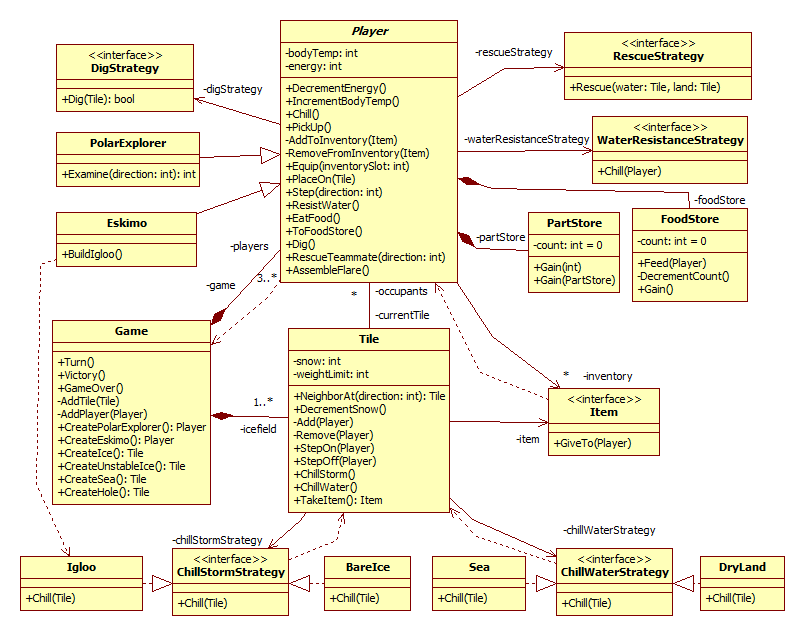
\includegraphics[angle=90, scale=0.76]{chapters/chapter04/ClassDiagramPart1.png}
		\caption{Osztálydiagram 1.}
		\label{fig:OsztalyDiagramPart1}
	\end{center}
\end{figure}
\begin{figure}[H]
	\begin{center}
		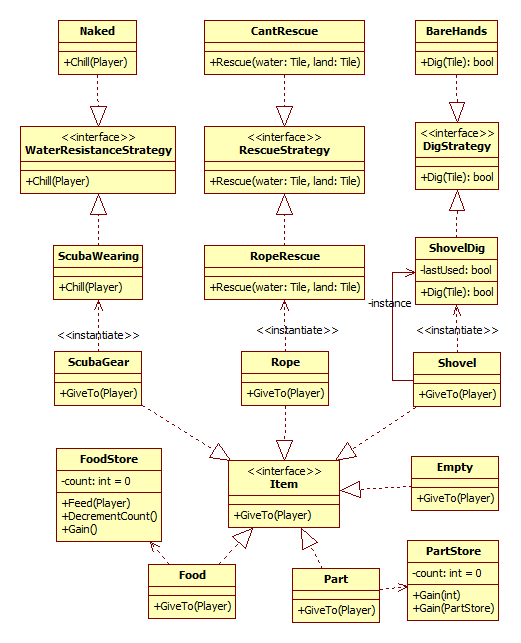
\includegraphics[width=17cm]{chapters/chapter04/ClassDiagramPart2.png}
		\caption{Osztálydiagram 2.}
		\label{fig:OsztalyDiagramPart2}
	\end{center}
\end{figure}

%\newpage
\section{Szekvencia diagramok}
%find . -printf "\\\begin{figure}[H]\n\t\\\begin{center}\n\t\t\\\includegraphics[width=10cm]{chapters/chapter04/seqdiag/%f}\n\t\t\\\caption{aaa}\n\t\t\\\label{bbb}\n\t\\\end{center}\n\\\end{figure}\n"

\begin{figure}[H]
	\begin{center}
		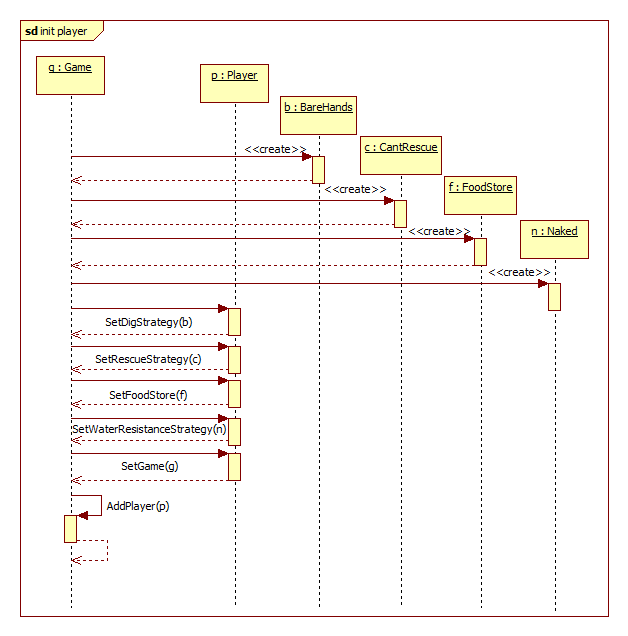
\includegraphics[width=15cm]{chapters/chapter04/seqdiag/Game_init_player.png}
		\caption{Game.CreateEskimo(), Game.CreatePolarExplorer()}
		\label{fig:GameInitPlayer}
	\end{center}
\end{figure}
\begin{figure}[H]
	\begin{center}
		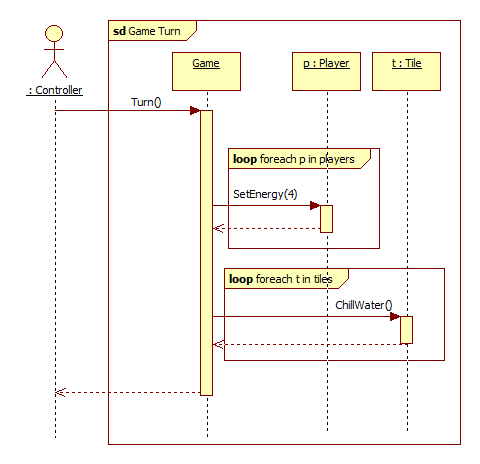
\includegraphics[width=10cm]{chapters/chapter04/seqdiag/Game_Turn.png}
		\caption{Game.Turn()}
		\label{fig:GameTurn}
	\end{center}
\end{figure}
\begin{figure}[H]
	\begin{center}
		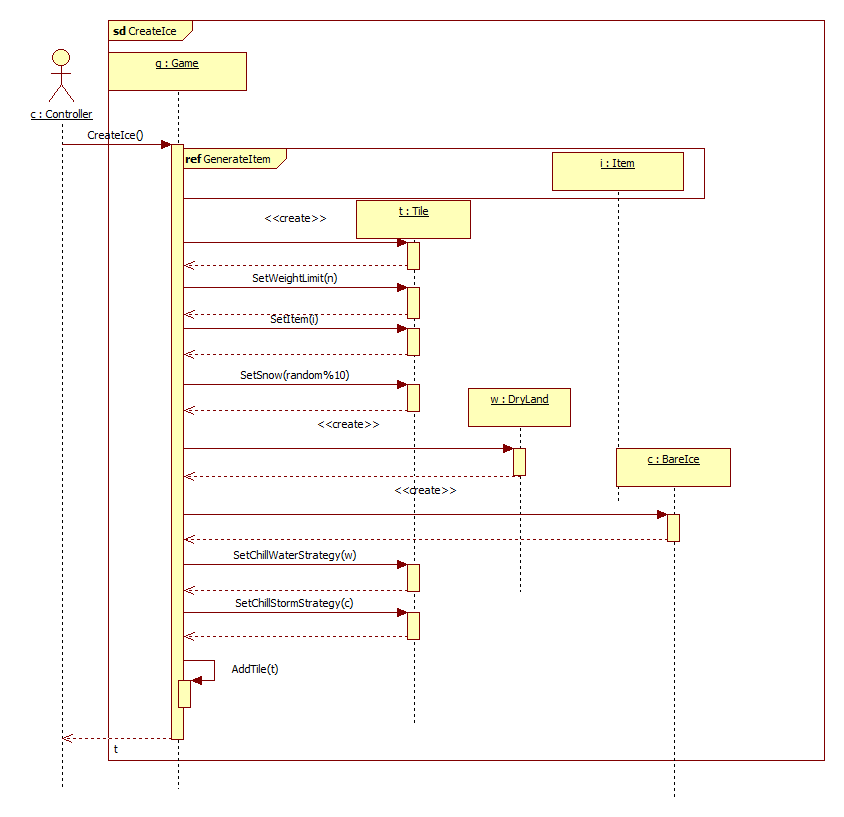
\includegraphics[width=15cm]{chapters/chapter04/seqdiag/Game_CreateIce.png}
		\caption{Game.CreateIce()}
		\label{fig:GameCreateIce}
	\end{center}
\end{figure}
\begin{figure}[H]
	\begin{center}
		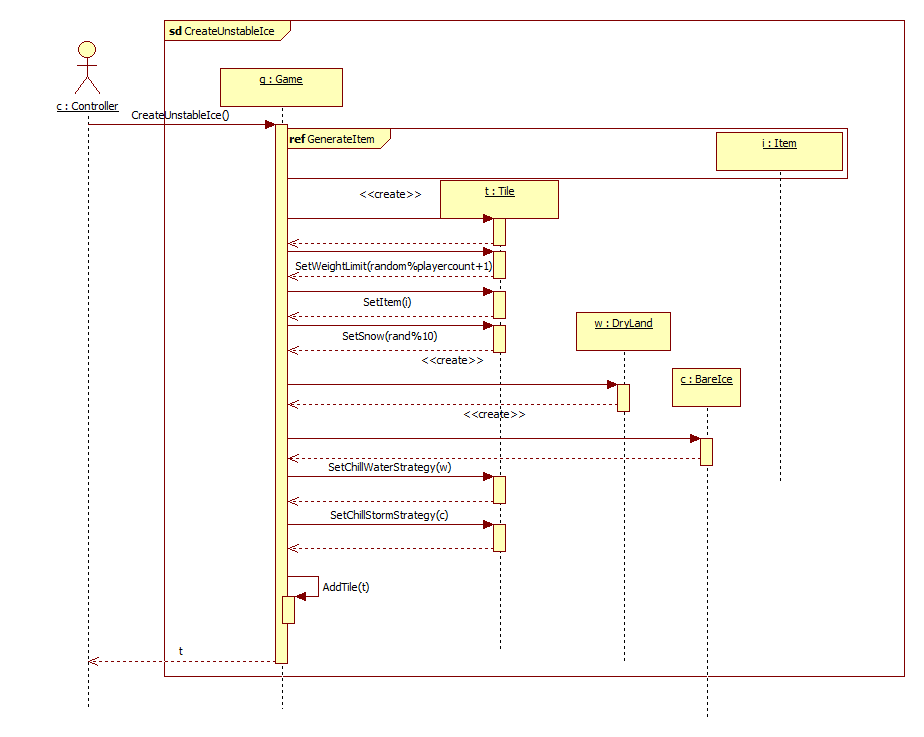
\includegraphics[width=17cm]{chapters/chapter04/seqdiag/Game_CreateUnstableIce.png}
		\caption{Game.CreateUnstableIce()}
		\label{fig:GameCreateUnstableIce}
	\end{center}
\end{figure}
\begin{figure}[H]
	\begin{center}
		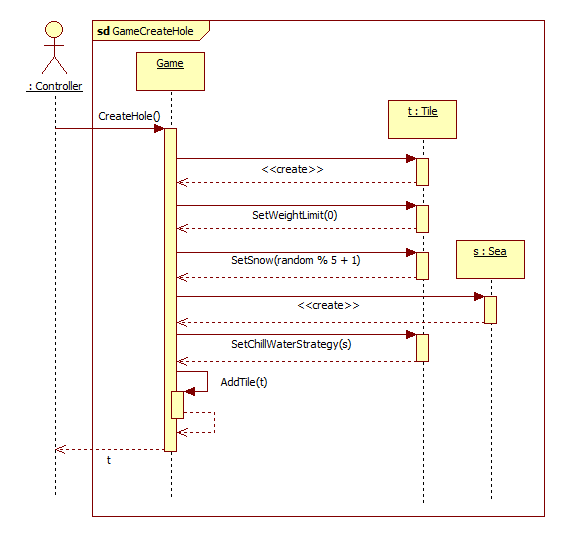
\includegraphics[width=15cm]{chapters/chapter04/seqdiag/Game_CreateHole.png}
		\caption{Game.CreateHole()}
		\label{fig:GameCreateHole}
	\end{center}
\end{figure}
\begin{figure}[H]
	\begin{center}
		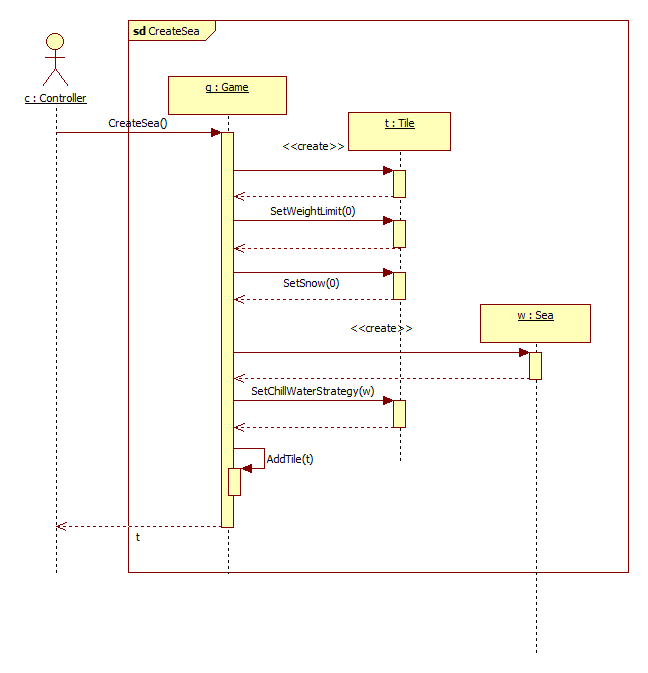
\includegraphics[width=13cm]{chapters/chapter04/seqdiag/Game_CreateSea.png}
		\caption{Game.CreateSea()}
		\label{fig:GameCreateSea}
	\end{center}
\end{figure}
\begin{figure}[H]
	\begin{center}
		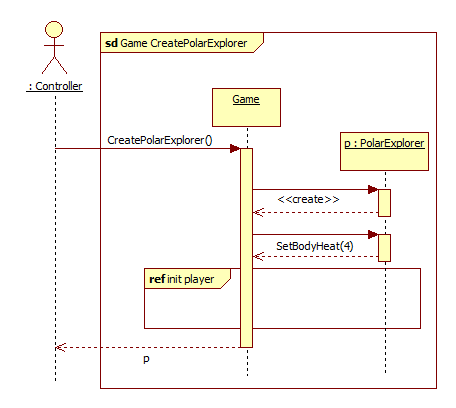
\includegraphics[width=10cm]{chapters/chapter04/seqdiag/Game_CreatePolarExplorer.png}
		\caption{Game.CreatePolarExplorer()}
		\label{fig:GameCreatePolarExplorer}
	\end{center}
\end{figure}
\begin{figure}[H]
	\begin{center}
		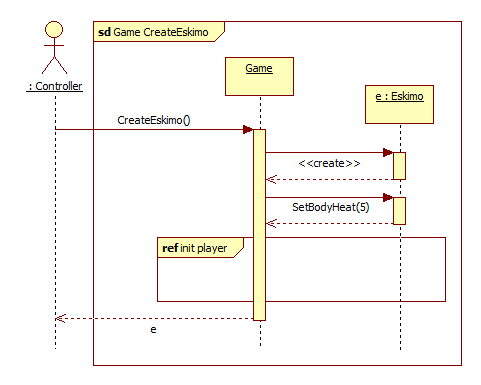
\includegraphics[width=10cm]{chapters/chapter04/seqdiag/Game_CreateEskimo.png}
		\caption{Game.CreateEskimo()}
		\label{fig:GameCreateEskimo}
	\end{center}
\end{figure}
\begin{figure}[H]
	\begin{center}
		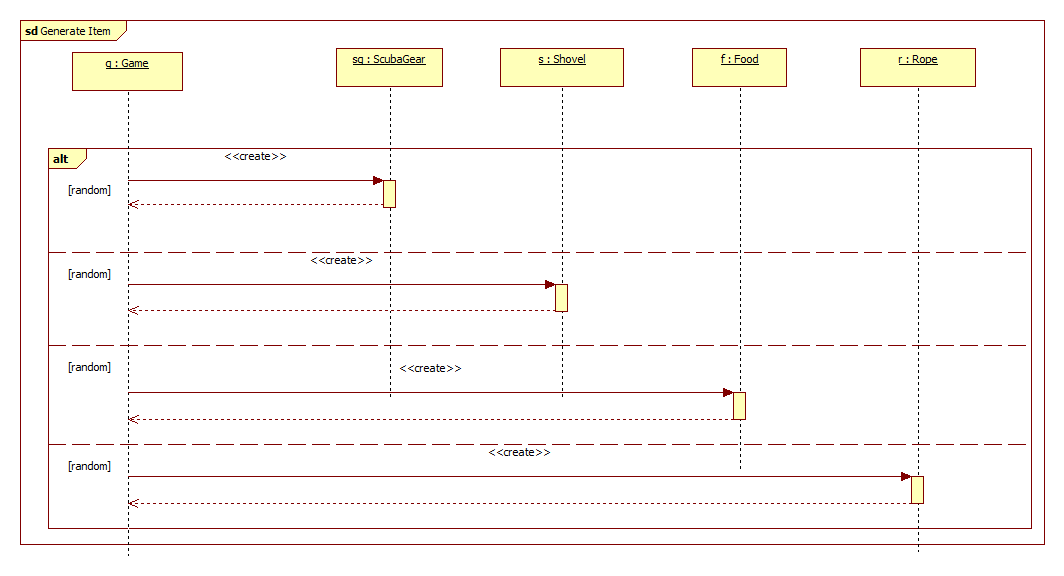
\includegraphics[width=17cm]{chapters/chapter04/seqdiag/Game_generate_item.png}
		\caption{Game.GenerateItem()}
		\label{fig:GameGenerateItem}
	\end{center}
\end{figure}
\begin{figure}[H]
	\begin{center}
		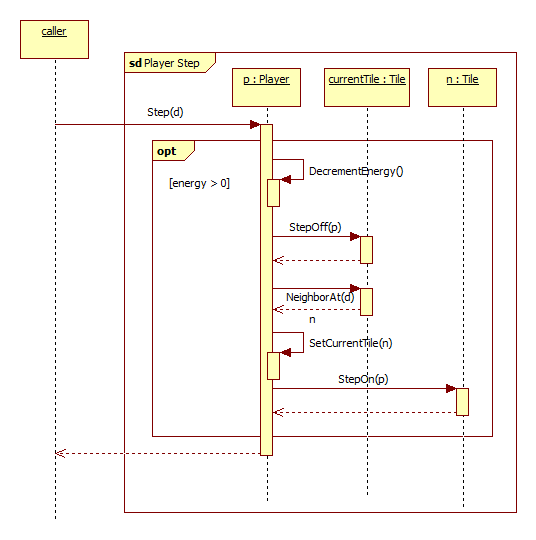
\includegraphics[width=11cm]{chapters/chapter04/seqdiag/Player_Step.png}
		\caption{Player.Step(direction: int)}
		\label{fig:PlayerStep}
	\end{center}
\end{figure}
\begin{figure}[H]
	\begin{center}
		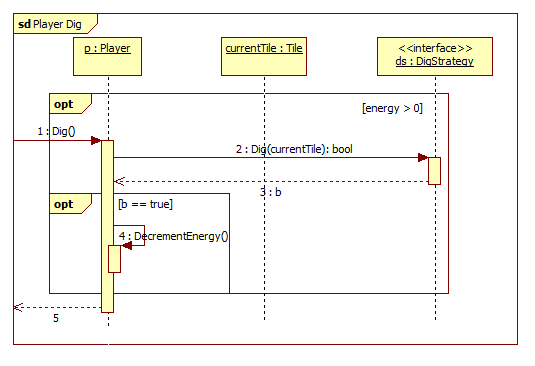
\includegraphics[width=15cm]{chapters/chapter04/seqdiag/Player_Dig.png}
		\caption{Player.Dig()}
		\label{fig:PlayerDig}
	\end{center}
\end{figure}
\begin{figure}[H]
	\begin{center}
		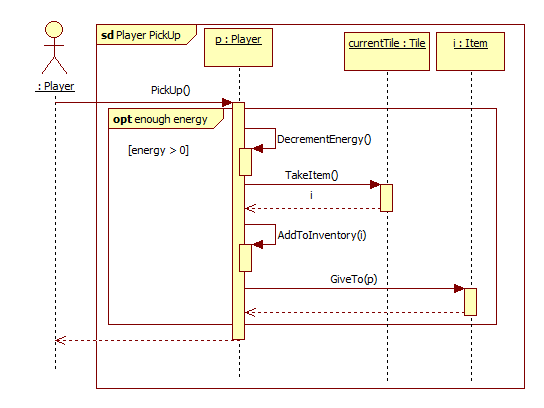
\includegraphics[width=15cm]{chapters/chapter04/seqdiag/Player_PickUp.png}
		\caption{Player.PickUp()}
		\label{fig:PlayerPickUp}
	\end{center}
\end{figure}
\begin{figure}[H]
	\begin{center}
		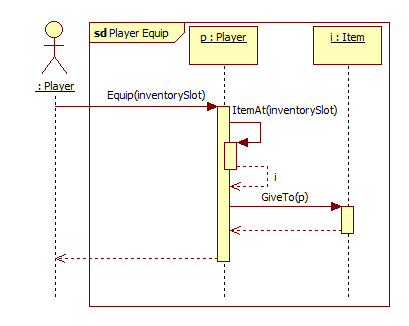
\includegraphics[width=15cm]{chapters/chapter04/seqdiag/Player_Equip.png}
		\caption{Player.Equip(int)}
		\label{fig:PlayerEquip}
	\end{center}
\end{figure}
\begin{figure}[H]
	\begin{center}
		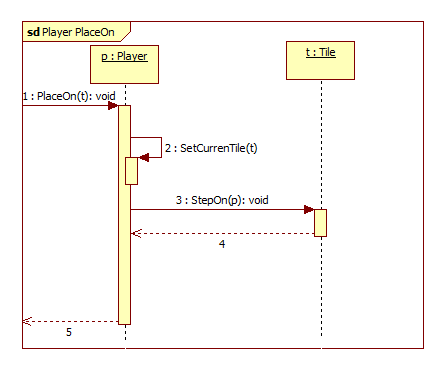
\includegraphics[width=10cm]{chapters/chapter04/seqdiag/Player_PlaceOn.png}
		\caption{Player.PlaceOn(Tile)}
		\label{fig:PlayerPlaceOn}
	\end{center}
\end{figure}
\begin{figure}[H]
	\begin{center}
		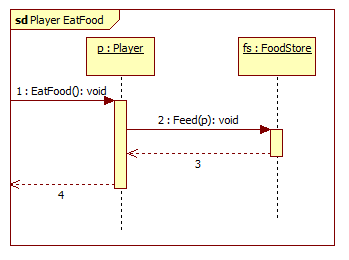
\includegraphics[width=10cm]{chapters/chapter04/seqdiag/Player_EatFood.png}
		\caption{Player.EatFood()}
		\label{fig:PlayerEatFood}
	\end{center}
\end{figure}
\begin{figure}[H]
	\begin{center}
		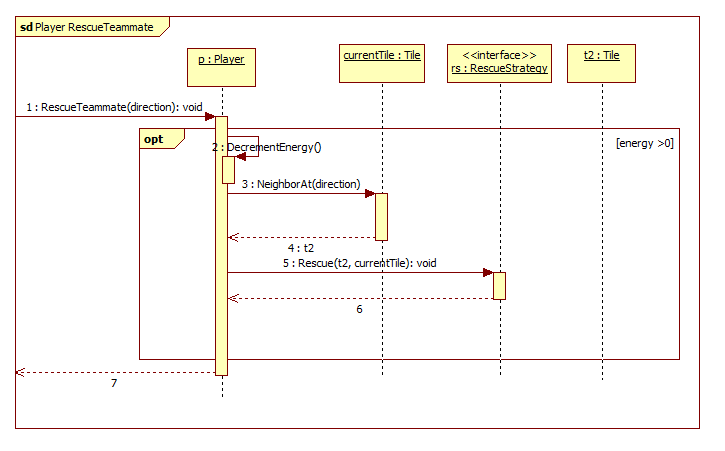
\includegraphics[width=15cm]{chapters/chapter04/seqdiag/Player_RescueTeammate.png}
		\caption{Player.RescueTeammate(direction: int)}
		\label{fig:Player.RescueTeammate}
	\end{center}
\end{figure}
\begin{figure}[H]
	\begin{center}
		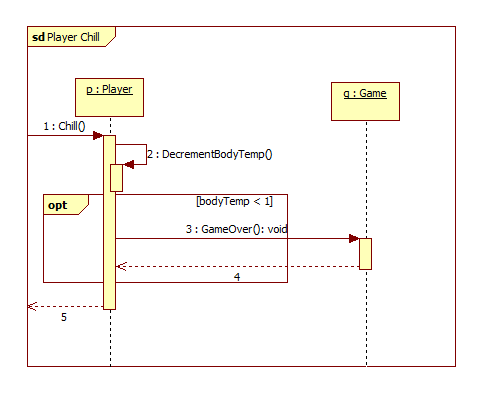
\includegraphics[width=10cm]{chapters/chapter04/seqdiag/Player_Chill.png}
		\caption{Player.Chill()}
		\label{fig:PlayerChill}
	\end{center}
\end{figure}
\begin{figure}[H]
	\begin{center}
		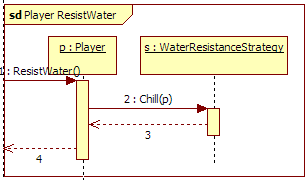
\includegraphics[width=10cm]{chapters/chapter04/seqdiag/Player_ResistWater.png}
		\caption{Player.ResistWater()}
		\label{fig:PlayerResistWater}
	\end{center}
\end{figure}
\begin{figure}[H]
	\begin{center}
		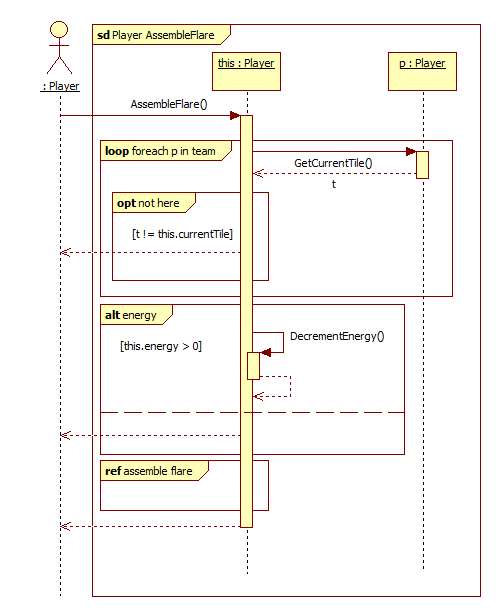
\includegraphics[width=10cm]{chapters/chapter04/seqdiag/Player_AssembleFlare.png}
		\caption{Player.AssembleFlare()}
		\label{fig:PlayerAssembleFlare}
	\end{center}
\end{figure}
\begin{figure}[H]
	\begin{center}
		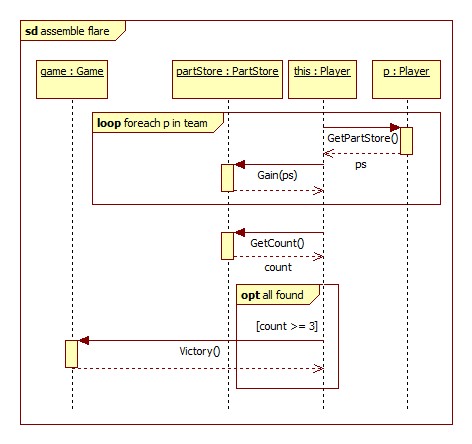
\includegraphics[width=10cm]{chapters/chapter04/seqdiag/Player_assemble_flare.png}
		\caption{Player.AssembleFlare()}
		\label{fig:PlayerAssembleFlare2}
	\end{center}
\end{figure}
\begin{figure}[H]
	\begin{center}
		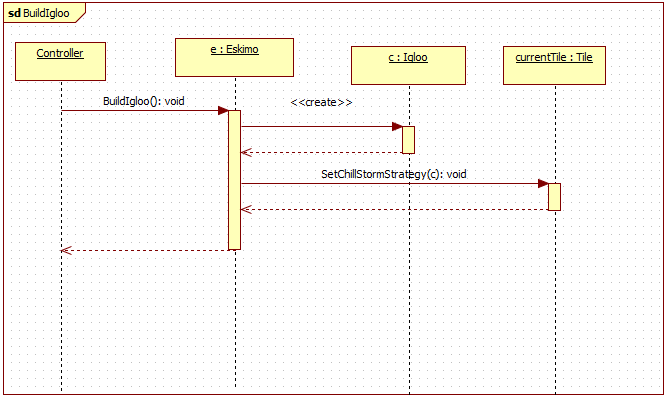
\includegraphics[width=15cm]{chapters/chapter04/seqdiag/Eskimo_BuildIgloo.png}
		\caption{Eskimo.BuildIgloo()}
		\label{fig:EskimoBuildIgloo}
	\end{center}
\end{figure}
\begin{figure}[H]
	\begin{center}
		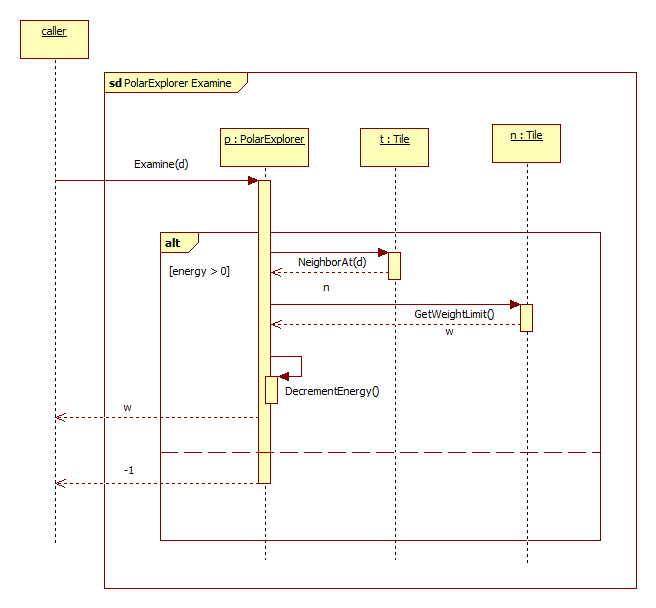
\includegraphics[width=15cm]{chapters/chapter04/seqdiag/PolarExplorer_Examine.png}
		\caption{PolarExplorer.Examine(direction: int)}
		\label{fig:PolarExplorerExamine}
	\end{center}
\end{figure}
\begin{figure}[H]
	\begin{center}
		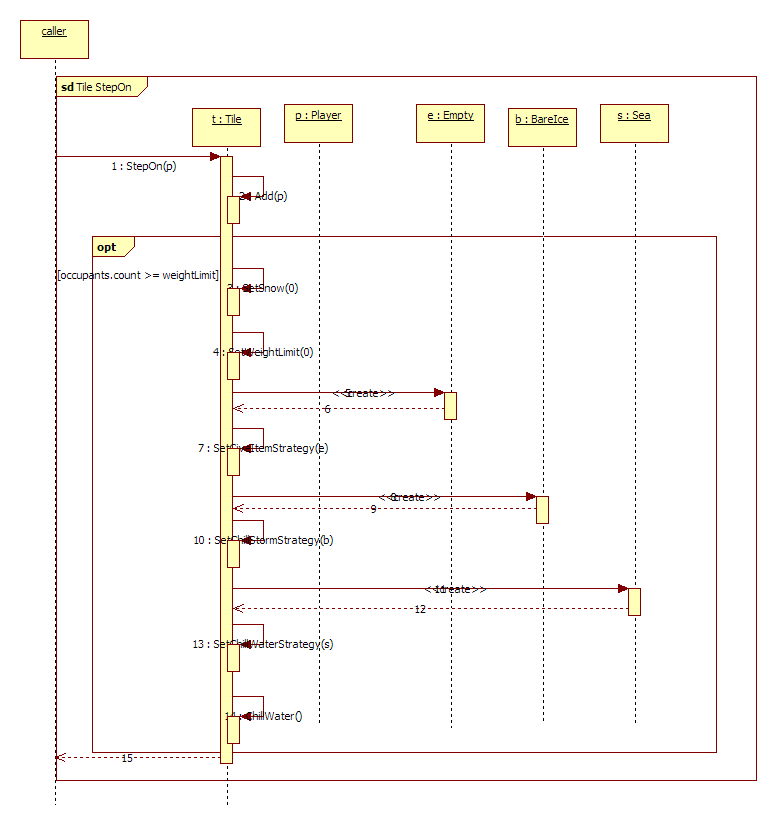
\includegraphics[width=15cm]{chapters/chapter04/seqdiag/Tile_StepOn.png}
		\caption{Tile.StepOn(Player)}
		\label{fig:TileStepOn}
	\end{center}
\end{figure}
\begin{figure}[H]
	\begin{center}
		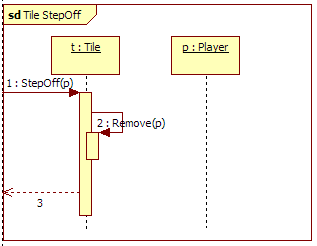
\includegraphics[width=10cm]{chapters/chapter04/seqdiag/Tile_StepOff.png}
		\caption{Tile.StepOff(Player)}
		\label{fig:TileStepOff}
	\end{center}
\end{figure}
\begin{figure}[H]
	\begin{center}
		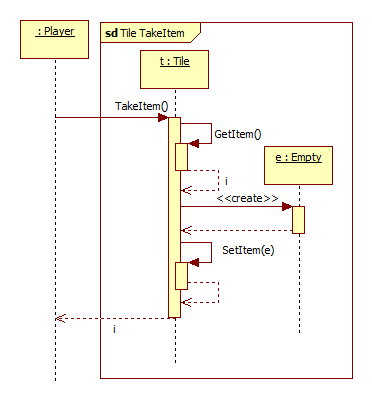
\includegraphics[width=14cm]{chapters/chapter04/seqdiag/Tile_TakeItem.png}
		\caption{Tile.TakeItem()}
		\label{fig:TileTakeItem}
	\end{center}
\end{figure}
\begin{figure}[H]
	\begin{center}
		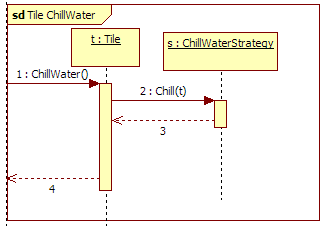
\includegraphics[width=10cm]{chapters/chapter04/seqdiag/Tile_ChillWater.png}
		\caption{Tile.ChillWater()}
		\label{fig:TileChillWater}
	\end{center}
\end{figure}
\begin{figure}[H]
	\begin{center}
		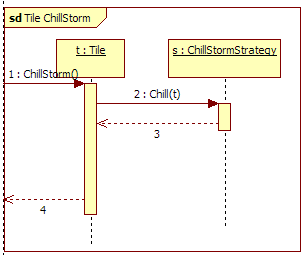
\includegraphics[width=10cm]{chapters/chapter04/seqdiag/Tile_ChillStorm.png}
		\caption{Tile.ChillStorm()}
		\label{fig:TileChillStorm}
	\end{center}
\end{figure}
\begin{figure}[H]
	\begin{center}
		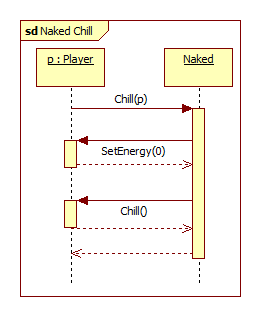
\includegraphics[width=10cm]{chapters/chapter04/seqdiag/Naked_Chill.png}
		\caption{Naked.Chill(Player)}
		\label{fig:NakedChill}
	\end{center}
\end{figure}
\begin{figure}[H]
	\begin{center}
		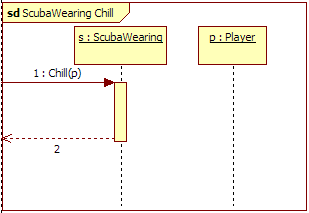
\includegraphics[width=10cm]{chapters/chapter04/seqdiag/ScubaWearing_Chill.png}
		\caption{ScubaWearing.Chill(Player)}
		\label{fig:ScubaWearingChill}
	\end{center}
\end{figure}
\begin{figure}[H]
	\begin{center}
		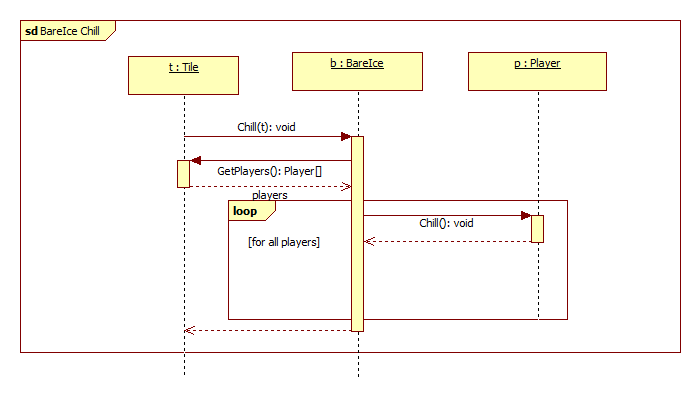
\includegraphics[width=15cm]{chapters/chapter04/seqdiag/BareIce_Chill.png}
		\caption{BareIce.Chill()}
		\label{fig:BareIceChill}
	\end{center}
\end{figure}
\begin{figure}[H]
	\begin{center}
		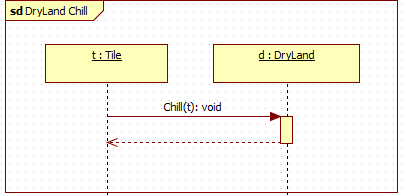
\includegraphics[width=10cm]{chapters/chapter04/seqdiag/DryLand_Chill.png}
		\caption{DryLand.Chill(Tile)}
		\label{fig:DryLandChill}
	\end{center}
\end{figure}
\begin{figure}[H]
	\begin{center}
		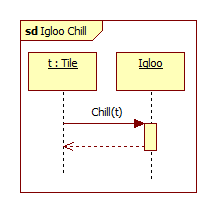
\includegraphics[width=10cm]{chapters/chapter04/seqdiag/Igloo_Chill.png}
		\caption{Igloo.Chill(Tile)}
		\label{fig:IglooChill}
	\end{center}
\end{figure}
\begin{figure}[H]
	\begin{center}
		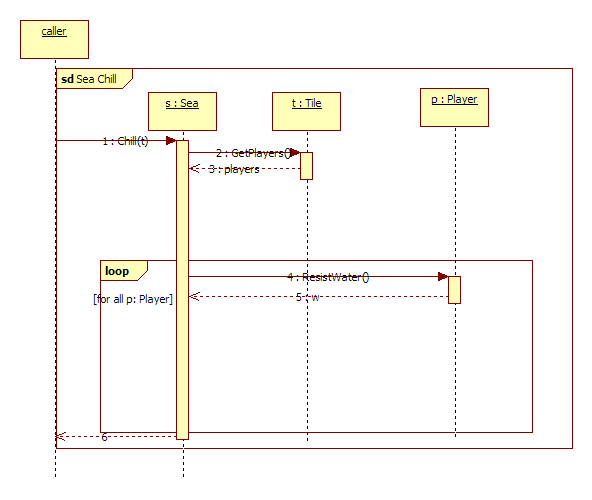
\includegraphics[width=13cm]{chapters/chapter04/seqdiag/Sea_Chill.png}
		\caption{Sea.Chill(Tile)}
		\label{fig:SeaChill}
	\end{center}
\end{figure}
\begin{figure}[H]
	\begin{center}
		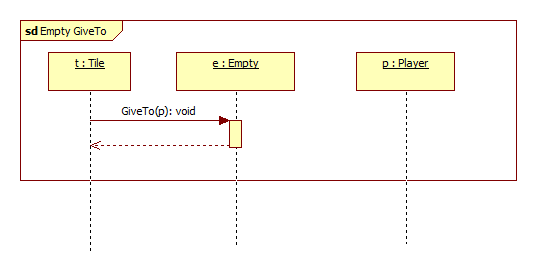
\includegraphics[width=13cm]{chapters/chapter04/seqdiag/Empty_GiveTo.png}
		\caption{Empty.GiveTo(Player)}
		\label{fig:EmptyGiveTo}
	\end{center}
\end{figure}
\begin{figure}[H]
	\begin{center}
		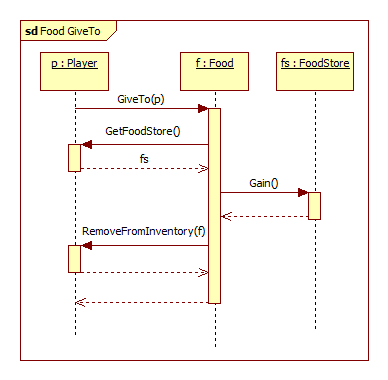
\includegraphics[width=15cm]{chapters/chapter04/seqdiag/Food_GiveTo.png}
		\caption{Food.GiveTo(Player)}
		\label{fig:FoodGiveTo}
	\end{center}
\end{figure}
\begin{figure}[H]
	\begin{center}
		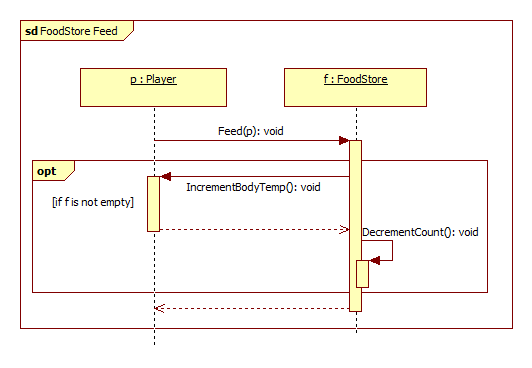
\includegraphics[width=12cm]{chapters/chapter04/seqdiag/FoodStore_Feed.png}
		\caption{FoodStore.Feed(Player)}
		\label{fig:FoodStoreFeed}
	\end{center}
\end{figure}
\begin{figure}[H]
	\begin{center}
		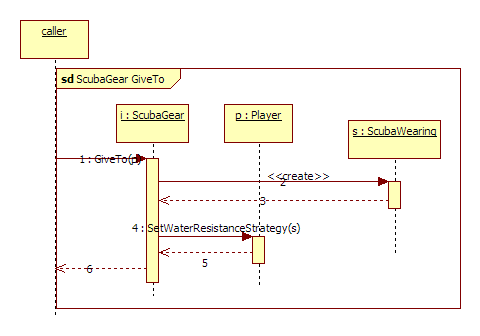
\includegraphics[width=10cm]{chapters/chapter04/seqdiag/ScubaGear_GiveTo.png}
		\caption{ScubaGear.GiveTo(Player)}
		\label{fig:ScubaGearGiveTo}
	\end{center}
\end{figure}
\begin{figure}[H]
	\begin{center}
		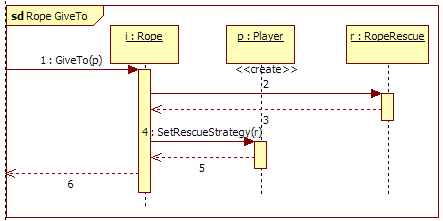
\includegraphics[width=10cm]{chapters/chapter04/seqdiag/Rope_GiveTo.png}
		\caption{Rope.GiveTo(Player)}
		\label{fig:RopeGiveTo}
	\end{center}
\end{figure}
\begin{figure}[H]
	\begin{center}
		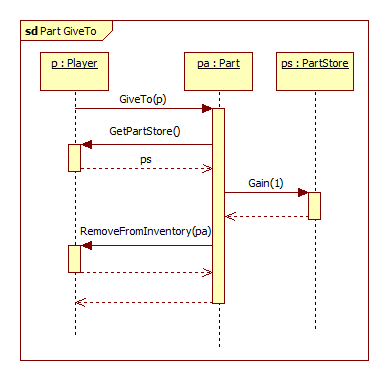
\includegraphics[width=10cm]{chapters/chapter04/seqdiag/Part_GiveTo.png}
		\caption{Part.GiveTo(Player)}
		\label{fig:PartGiveTo}
	\end{center}
\end{figure}
\begin{figure}[H]
	\begin{center}
		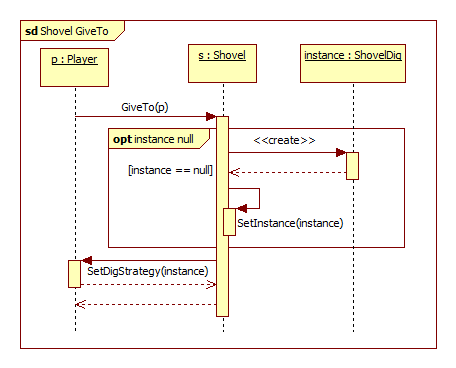
\includegraphics[width=10cm]{chapters/chapter04/seqdiag/Shovel_GiveTo.png}
		\caption{Shovel.GiveTo(Player)}
		\label{fig:ShovelGiveTo}
	\end{center}
\end{figure}
\begin{figure}[H]
	\begin{center}
		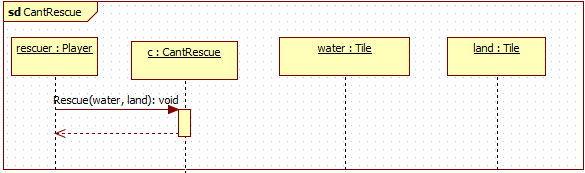
\includegraphics[width=13cm]{chapters/chapter04/seqdiag/CantRescue_Rescue.png}
		\caption{CantRescue.Rescue(Tile, Tile)}
		\label{fig:CantRescueRescue}
	\end{center}
\end{figure}
\begin{figure}[H]
	\begin{center}
		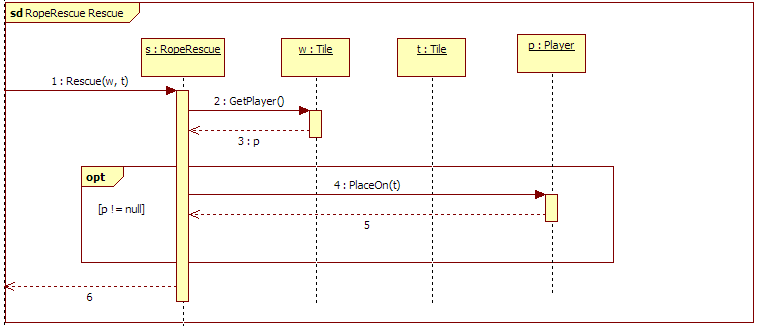
\includegraphics[width=13cm]{chapters/chapter04/seqdiag/RopeRescue_Rescue.png}
		\caption{RopeRescue.Rescue(Tile, Tile)}
		\label{fig:RopeRescueRescue}
	\end{center}
\end{figure}
\begin{figure}[H]
	\begin{center}
		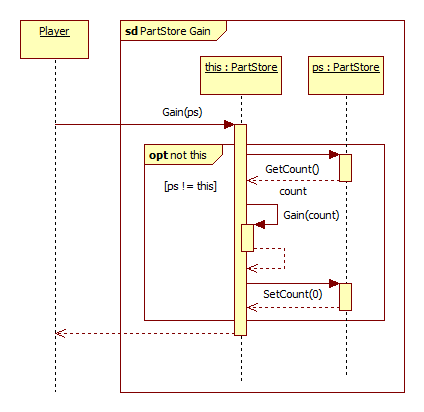
\includegraphics[width=10cm]{chapters/chapter04/seqdiag/PartStore_Gain.png}
		\caption{PartStore.Gain(PartStore)}
		\label{fig:PartStoreGain}
	\end{center}
\end{figure}
\begin{figure}[H]
	\begin{center}
		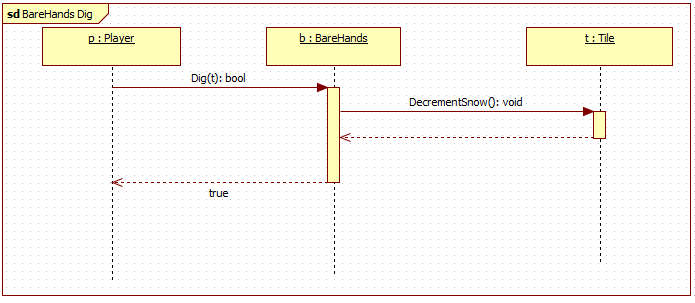
\includegraphics[width=15cm]{chapters/chapter04/seqdiag/BareHandsDig_Dig.png}
		\caption{BareHandsDig.Dig(Tile)}
		\label{fig:BareHandsDig.Dig}
	\end{center}
\end{figure}
\begin{figure}[H]
	\begin{center}
		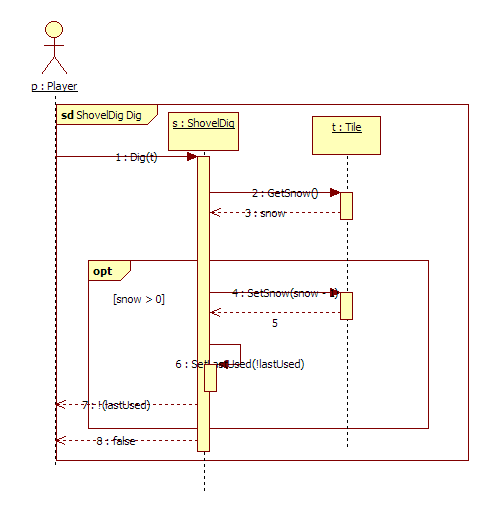
\includegraphics[width=10cm]{chapters/chapter04/seqdiag/ShovelDig_Dig.png}
		\caption{ShovelDig.Dig(Tile)}
		\label{fig:ShovelDigDig}
	\end{center}
\end{figure}
